% ══════════════════════════════════════════════════════════════
\section{Credential Ladder Detail}
\label{app:credentials}

Table~\ref{tab:credential-treadmill} gives the full credential ladder summarized in Figure~\ref{fig:credentials}.

\begin{table}[!htbp]
\centering
\small
\caption{Credential ladder. The OpenAlex long-tail researcher cohort ($n = 771$, citations $500$--$30{,}000$) supplies the working-researcher baseline. The two rows marked $\dagger$ are large-team co-authorship cohorts shown for context, not credentials, and are excluded from the ``$7$ of $9$'' count.}
\label{tab:credential-treadmill}
\begin{tabular}{lrrr}
\toprule
Credential & $n$ & Mean NameRank & vs.\ baseline \\
\midrule
ICPC World Finalist gold & 18 & 0.610 & $+0.146$ \\
Putnam top-25 fellow & 35 & 0.608 & $+0.144$ \\
\textbf{OpenAlex long-tail researchers (baseline)} & \textbf{771} & \textbf{0.464} & --- \\
NOI China gold & 29 & 0.368 & $-0.096$ \\
\textbf{IMO gold (2005--2015)} & \textbf{197} & \textbf{0.362} & $\mathbf{-0.102}$ \\
MSRA PhD Fellowship & 237 & 0.343 & $-0.121$ \\
IOI gold & 68 & 0.341 & $-0.123$ \\
Rhodes Scholarship & 36 & 0.315 & $-0.149$ \\
CMO China gold & 131 & 0.302 & $-0.162$ \\
CPhO China first prize & 50 & 0.182 & $-0.282$ \\
DeepSeek-V3 paper author$^\dagger$ & 69 & 0.178 & $-0.286$ \\
GPT-5 system-card author$^\dagger$ & 80 & 0.042 & $-0.422$ \\
\bottomrule
\end{tabular}
\end{table}

\textbf{Career-track split.} Within IMO gold medalists, US-tracked academic/industry careers---the subset most comparable to the citation-floored OpenAlex baseline---score ${\sim}0.50$; non-Anglophone-tracked golds score ${\sim}0.30$. The medal-and-name pair propagates only where the post-medal career produces English text.

\textbf{Temporal patterns.} Within MSRA fellows, five-year-cohort means rise from $0.312$ (2005--2009) to $0.337$ (2010--2014) to $0.382$ (2015--2019) and dip to $0.343$ (2020--2024), consistent with recent fellows having had less time for post-fellowship production to propagate. Within IMO 2005--2015, Pearson(year, NameRank) $= -0.042$, indistinguishable from zero: the credential signal neither strengthens nor decays within the ten-year window.

% ══════════════════════════════════════════════════════════════
\section{Conditional-Probe Asymmetry Details}
\label{app:asymmetry}

For each of the $11$ verified (creator, artifact) pairs, the full per-model breakdown of $C\!\to\!A$ and $A\!\to\!C$ (fraction of non-refusal model responses that name the counterpart) is released as a supplementary CSV.

\textbf{Per-model mention table for Jiayi Weng / Tianshou.} Of the $28$ non-refusal responses to ``tell me about Jiayi Weng,'' $7$ name Tianshou: claude-opus-4.6-think, claude-sonnet-4.6-think, gemini-3-flash-think, gemini-3.1-pro, glm-5.1-think, gpt-5.5-think, kimi-k2.6-think. All other models that respond do not name Tianshou. The $7$ mentioning models have judge scores ranging $0.70$ to $0.80$ (mean $0.71$); the $21$ non-mentioning responding models range $0.00$ to $0.50$ (mean $0.35$). The score lift from artifact-mention is $+0.36$.

% ══════════════════════════════════════════════════════════════
\section{Cross-Language and East--West Detail}
\label{app:cross-lang}

\textbf{Sub-run cohort selection.} The Chinese-prompt sub-run covers $240$ entities: the full diagnostic reference set ($37$), all NOI China gold medalists ($29$), all DeepSeek-V3 paper authors ($69$), $30$ random samples each from the CMO, CPhO, and MSRA Fellowship cohorts, and $5$ each from the writer, filmmaker, and politician cohorts as Western controls---$240 \times 37 = 8{,}880$ records.

\textbf{English-prompt East--West extremes.} On English prompts, the strongest Chinese-panel lifts over the Western panel are Chinese-content entities: Wei Dongyi (Chinese mathematics figure; Chinese-panel mean $0.80$ vs.\ Western $0.53$) and Zhang Fang (NOI gold; $0.45$ vs.\ $0.20$). The strongest Western-panel lifts are non-Chinese names on which Chinese models refuse: Saad Albawi ($0.59$ Western vs.\ $0.16$ Chinese) and Qingzi Vera Liao (Chinese-name CS faculty at a Western institution; $0.50$ vs.\ $0.15$).

\textbf{Per-model prompt-language deltas.} The Chinese-prompt shift is universal rather than vendor-specific: models gaining on Chinese prompts include Western (claude-sonnet-4.6-think $+0.17$, gemini-3.1-pro $+0.12$, gemma-3-12b $+0.12$) and Chinese (deepseek-v4-pro-think $+0.14$, qwen3-235b $+0.10$) models, and models losing include both classes as well (llama-4-maverick $-0.20$, gpt-5.4 $-0.12$, glm-4-32b $-0.05$, kimi-k2 $-0.05$). The class averages are $+0.014$ (Western) and $+0.028$ (Chinese): both lift slightly, and the dominant signal is entity-name match, not model origin.

\textbf{Per-entity deltas.} The full per-entity $\Delta(\mathrm{NR}_\mathrm{zh} - \mathrm{NR}_\mathrm{en})$ table is released as a supplementary CSV. Selected diagnostic entries (the largest suppressions beyond the table: Leng Junsheng $-0.17$, Du Zhuofan $-0.15$, Aleksander Madry $-0.12$):

\begin{center}
\small
\begin{tabular}{lrrrr}
\toprule
Entity & $\mathrm{NR}_\mathrm{en}$ & $\mathrm{NR}_\mathrm{zh}$ & $\Delta$ & Cohort \\
\midrule
Jiayi Weng & 0.331 & 0.327 & $-0.004$ & reference set \\
Tianshou & 0.420 & 0.399 & $-0.021$ & reference set \\
tuixue.online & 0.250 & 0.262 & $+0.012$ & reference set \\
Andrej Karpathy & 0.614 & 0.549 & $-0.066$ & reference set \\
Tri Dao & 0.532 & 0.488 & $-0.044$ & reference set \\
FlashAttention & 0.607 & 0.470 & $-0.137$ & reference set \\
Bojie Li & 0.090 & 0.105 & $+0.014$ & reference set \\
\midrule
Wang Haoyu (Wang Hao-yu) & 0.260 & 0.430 & $+0.170$ & CMO China gold \\
Yao Xuanrong (Yao Xuan-rong) & 0.250 & 0.420 & $+0.160$ & NOI China gold \\
Wang Zhongjian (Wang Zhong-jian) & 0.260 & 0.420 & $+0.160$ & CMO China gold \\
Zijia Zhu & 0.100 & 0.290 & $+0.190$ & DeepSeek-V3 author \\
Peng Zhang & 0.160 & 0.330 & $+0.170$ & DeepSeek-V3 author \\
\bottomrule
\end{tabular}
\end{center}

The pattern is consistent: Chinese-character names lift on Chinese prompts; English-coded artifacts lose on Chinese prompts; flat-cross-language entities have name attribution roughly equal in both training corpora.

% ══════════════════════════════════════════════════════════════
\section{External Validity Regressions}
\label{app:external}

Full regression results for NameRank on external impact metrics, restricted to the OpenAlex long-tail researcher cohort ($n = 771$, citations $500$--$30{,}000$, $h$-index from OpenAlex).

\begin{center}
\small
\begin{tabular}{lrr}
\toprule
Predictor set & Full-sample $R^2$ & $10$-fold CV $R^2$ (mean $\pm$ sd) \\
\midrule
$\log(\text{citations})$ & 0.137 & $0.12 \pm 0.07$ \\
$\log(h\text{-index})$ & 0.398 & $0.38 \pm 0.09$ \\
$\log(\text{citations}) + \log(h\text{-index})$ & 0.398 & $0.38 \pm 0.09$ \\
\bottomrule
\end{tabular}
\end{center}

Cross-validation is repeated $10$-fold ($20$ repeats, $200$ folds, fixed seed); the $\pm$ is the across-fold standard deviation. We use repeated CV rather than a single $70/30$ split because at $n = 771$ a single split's held-out $R^2$ varies by ${\sim}0.15$ across seeds (one favorable split gave $0.50$), which would overstate generalization. The marginal $R^2$ of $\log(\text{citations})$ given $\log(h\text{-index})$ is $0.000$; the coefficient on $\log(\text{citations})$ in joint regression is $-0.002$, indistinguishable from zero, and citations add no held-out signal.

\textbf{Decile breakdown of NameRank by $h$-index} (Table~\ref{tab:h-index-decile}):

\begin{table}[!htbp]
\centering
\small
\caption{Mean NameRank by $h$-index decile within OpenAlex long-tail researchers.}
\label{tab:h-index-decile}
\begin{tabular}{rrrr}
\toprule
Decile & $n$ & Mean $h$ & Mean NameRank \\
\midrule
D1 & 77 & 2.9 & 0.219 \\
D2 & 77 & 8.1 & 0.329 \\
D3 & 77 & 12.4 & 0.392 \\
D4 & 77 & 16.7 & 0.448 \\
D5 & 77 & 20.9 & 0.464 \\
D6 & 77 & 25.8 & 0.524 \\
D7 & 77 & 30.6 & 0.539 \\
D8 & 77 & 36.9 & 0.574 \\
D9 & 77 & 45.4 & 0.546 \\
D10 & 77 & 60.4 & 0.601 \\
\bottomrule
\end{tabular}
\end{table}

The relationship is near-monotonic (a single dip at D9) and saturates above $h \geq 40$. The bottom decile ($h < 5$) shows NameRank floored at $0.22$---the working-researcher floor, not zero.

% ══════════════════════════════════════════════════════════════
\section{Institution and Country Gradient Detail}
\label{app:geography}

Table~\ref{tab:cs-country} gives the full country-level aggregation behind Figure~\ref{fig:country}.

\begin{table}[!htbp]
\centering
\small
\caption{CS-faculty NameRank by country of institutional affiliation, for countries with $\geq 3$ sampled faculty. An \emph{Other/Unknown} bucket ($n=236$; CS-Rankings affiliations not matched by the keyword-prefix country lookup) is omitted. Only the USA ($n=302$), China ($30$), UK ($16$), Australia and Hong Kong ($11$), and Brazil and India ($10$) reach $n \geq 10$; the remaining rows are point estimates with wide intervals and should not be finely ranked against one another.}
\label{tab:cs-country}
\begin{tabular}{lrrrr}
\toprule
Country & $n$ & Mean & Median & frac $\geq 0.5$ \\
\midrule
Israel & 7 & 0.506 & 0.528 & 57\% \\
Singapore & 7 & 0.497 & 0.480 & 43\% \\
Sweden & 5 & 0.492 & 0.490 & 40\% \\
Germany & 9 & 0.490 & 0.488 & 44\% \\
Switzerland & 4 & 0.489 & 0.467 & 50\% \\
Canada & 9 & 0.478 & 0.463 & 22\% \\
USA & 302 & 0.460 & 0.488 & 46\% \\
Netherlands & 9 & 0.447 & 0.432 & 33\% \\
UK & 16 & 0.438 & 0.440 & 38\% \\
Hong Kong & 11 & 0.431 & 0.452 & 36\% \\
Portugal & 5 & 0.427 & 0.442 & 20\% \\
Brazil & 10 & 0.388 & 0.409 & 10\% \\
Australia & 11 & 0.341 & 0.291 & 18\% \\
France & 3 & 0.312 & 0.341 & 0\% \\
\textbf{China} & 30 & \textbf{0.311} & 0.285 & 7\% \\
Spain & 8 & 0.303 & 0.288 & 13\% \\
India & 10 & 0.292 & 0.279 & 0\% \\
\bottomrule
\end{tabular}
\end{table}

The well-sampled backbone of the gradient is USA (mean $0.460$, $95\%$ CI $[0.443, 0.476]$) against China ($0.311$, $[0.271, 0.350]$) and India ($0.292$, $[0.234, 0.351]$): the intervals do not overlap. The apparent leaders (Israel, Singapore, Sweden) sit above the USA in point estimate with intervals that overlap it, and are read as suggestive only.

% ══════════════════════════════════════════════════════════════
\section{Variance Decomposition: Per-Cohort Within-Entity Disagreement}
\label{app:variance}

The within-entity model-disagreement (standard deviation across the $37$-model panel for each entity, averaged within cohort) ranges over an order of magnitude, from $0.404$ (NOI China gold) down to $0.113$ (online courses); Figure~\ref{fig:app-sigma} gives the full ladder.

\textbf{Interpretation.} High within-entity $\sigma$ cohorts (NOI/ICPC/CMO/IMO/long-tail-OpenAlex) exhibit genuine corpus-pocket-specific recognition: different models trained on different fractions of available corpus see different fractions of the entity's coverage. Low within-entity $\sigma$ cohorts (online courses, conferences, named methods, books) have universal corpus presence: all models agree because the entity name appears in nearly every training-data source.

\begin{figure}[!htbp]
    \centering
    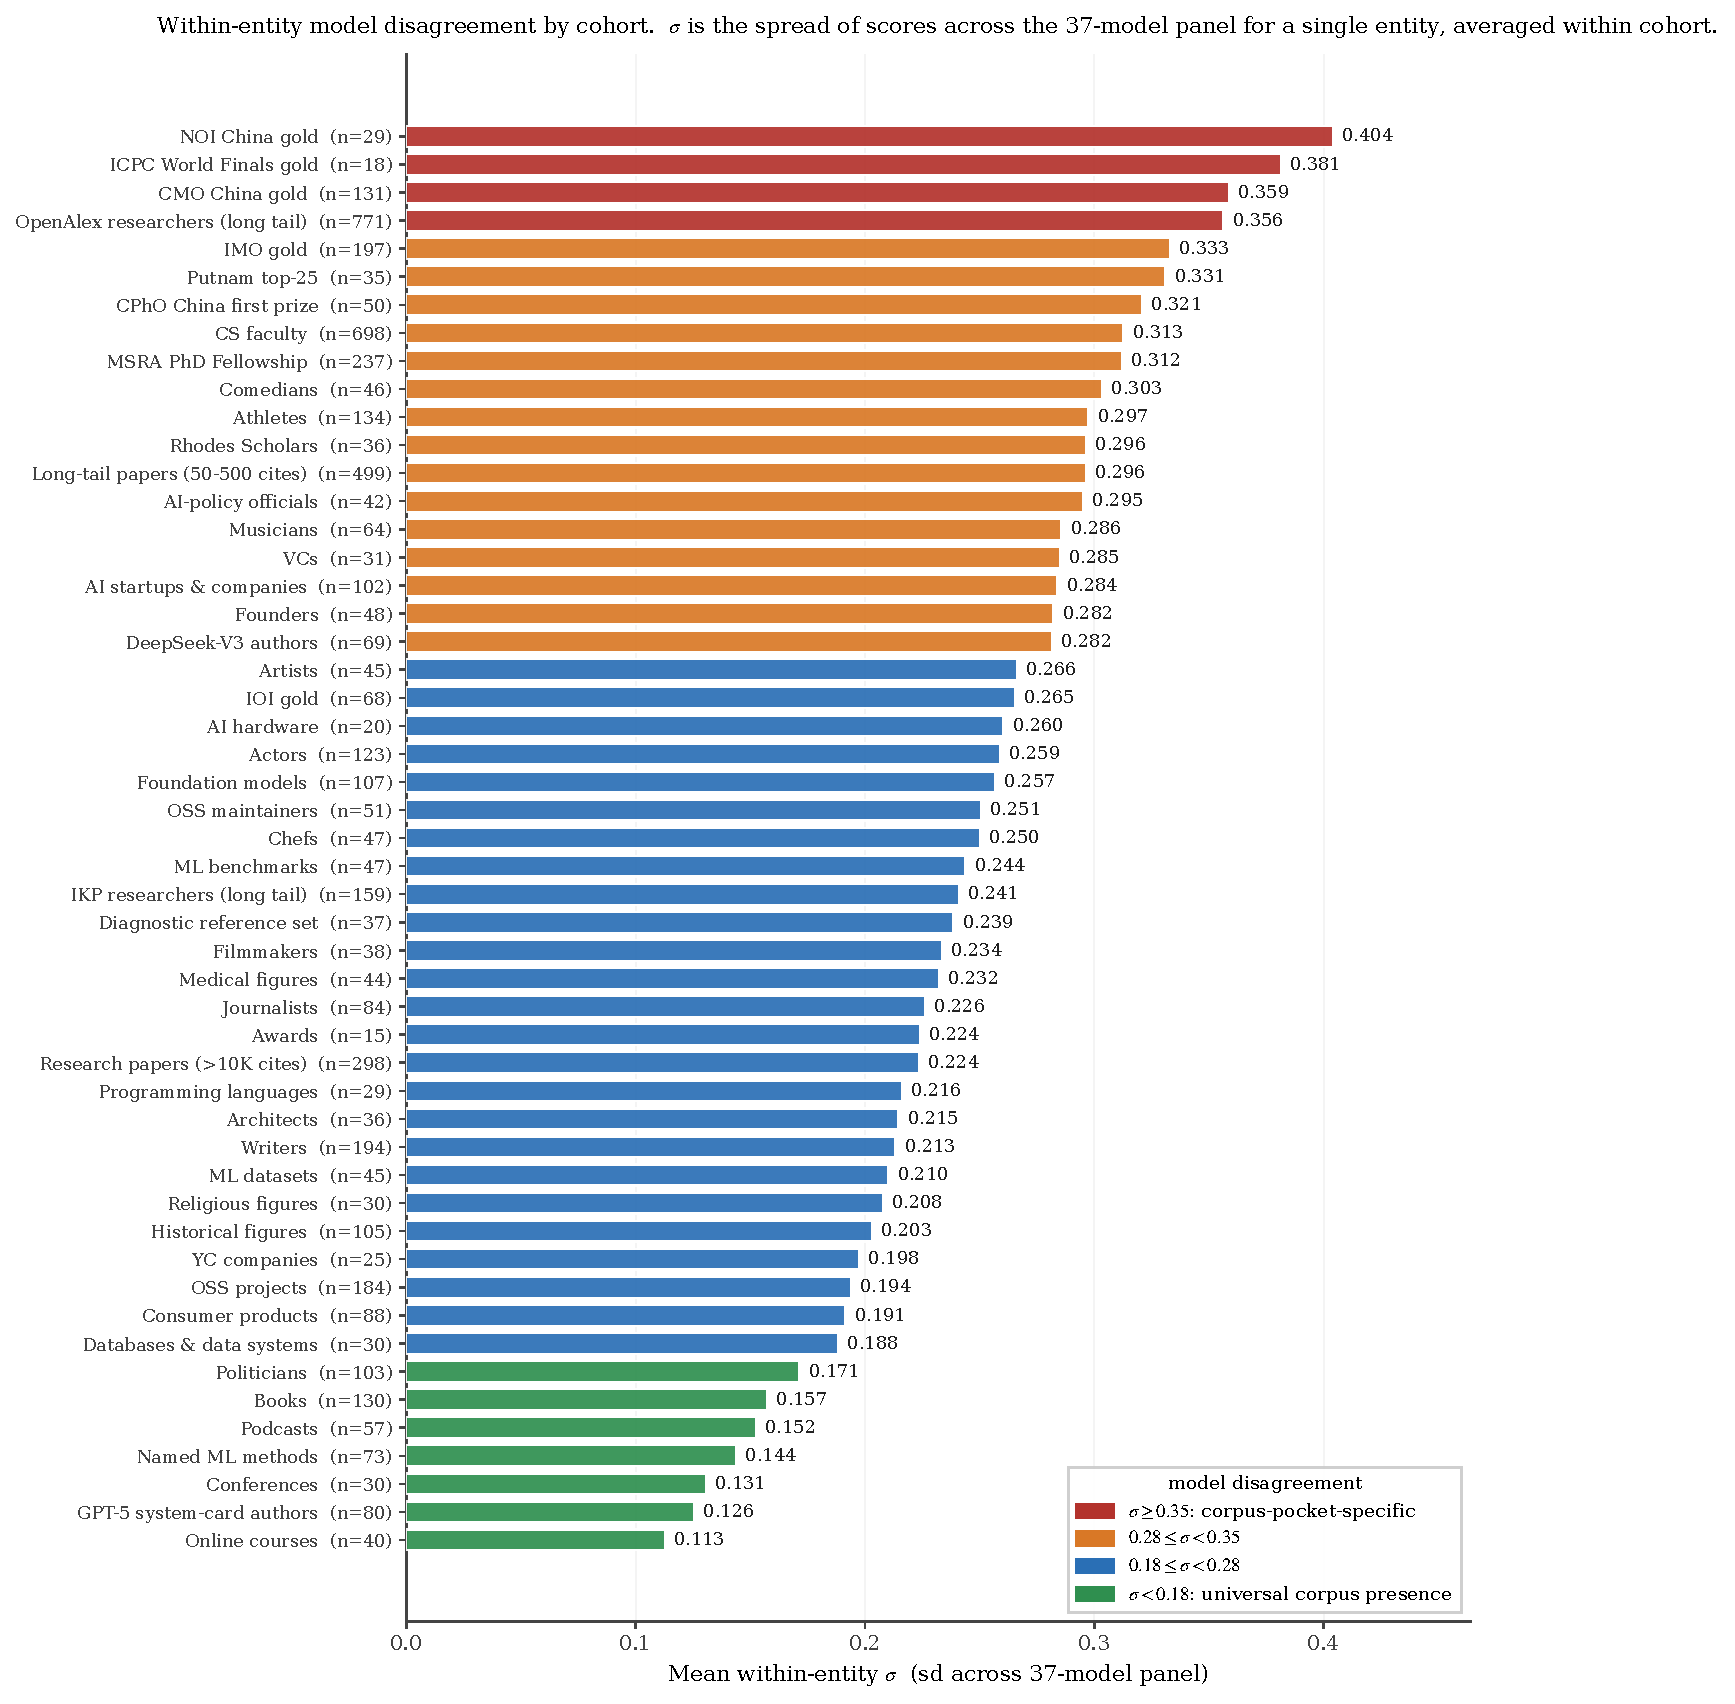
\includegraphics[width=0.92\textwidth]{figures/fig_app_sigma.pdf}
    \caption{Full within-entity $\sigma$ ladder across all cohorts with $n \geq 10$. Color bands group cohorts by the four $\sigma$ regimes (universal $\to$ corpus-pocket-specific). The high-$\sigma$ end is dominated by competition-credential and long-tail academic cohorts whose recognition is genuinely corpus-fragment-specific; the low-$\sigma$ end is dominated by entities whose names appear in nearly every training source (online courses, conferences, named methods, books).}
    \label{fig:app-sigma}
\end{figure}

The variance pattern is itself a probe of corpus-pocket distribution: cohorts with high $\sigma$ are the ones where ``which model do you ask?'' changes the answer.

% ══════════════════════════════════════════════════════════════
\section{Prompt-Paraphrase Sensitivity}
\label{app:prompt-sensitivity}

We re-probed a cohort-stratified $200$-entity subset ($30$ each from IMO gold, OpenAlex long-tail researchers, CS faculty, Writers, OSS projects, GPT-5 system-card authors; $10$ each from Research papers and Filmmakers) on the full $37$-model panel under three paraphrased probe templates (T1--T3) alongside the original (T0), for $29{,}600$ records. The four templates:

\begin{verbatim}
T0: Tell me what you know about {name}, who is {context}. If you do
    not recognize this entity, respond with "unknown". Limit your
    response to about 150 words.
T1: What can you tell me about {name}? They are {context}. Reply with
    only "unknown" if you are not familiar with this entity. Aim for
    about 150 words.
T2: Please share what you know about {name}, {context}. If unknown to
    you, answer with just "unknown". Keep it under ~150 words.
T3: Briefly describe {name}, who is {context}. Respond "unknown" if
    you have no information. Around 150 words please.
\end{verbatim}

\begin{table}[!htbp]
\centering
\small
\caption{Additive variance decomposition over the $29{,}600$ prompt-sensitivity records (entity, model, template, cohort as main effects). Template is the smallest main effect. The model share exceeds the full-panel $10.9\%$ (Section~\ref{sec:results-validation}) because this cohort-stratified subset over-represents silent and universal cohorts, compressing the entity-vs-model contrast; the valid within-experiment comparison is template ($1.78\%$) vs model ($26.5\%$).}
\label{tab:prompt-variance}
\begin{tabular}{lrr}
\toprule
Factor & SS & \% of total \\
\midrule
Entity & 985.3 & 24.19\% \\
Model & 1079.9 & 26.51\% \\
Cohort (entity-implied) & 551.9 & 13.55\% \\
\textbf{Template} & \textbf{72.4} & \textbf{1.78\%} \\
Residual (after entity+model+template) & 1936.3 & 47.53\% \\
\bottomrule
\end{tabular}
\end{table}

\begin{table}[!htbp]
\centering
\small
\caption{Cohort-mean NameRank under each template (sorted by T0). The ordering is preserved; T0 is systematically higher. Pairwise panel-mean Pearson across all six template pairs is $0.927$--$0.977$ (lowest: T0--T3); within-(entity, model) cross-template $\sigma$ has median $0.109$; the panel-mean variance across templates is $0.042\times$ the single-template cross-model variance.}
\label{tab:prompt-cohort-means}
\begin{tabular}{lrrrr}
\toprule
Cohort & T0 & T1 & T2 & T3 \\
\midrule
Filmmakers & 0.761 & 0.506 & 0.513 & 0.532 \\
Writers & 0.597 & 0.388 & 0.403 & 0.405 \\
Research papers & 0.581 & 0.391 & 0.394 & 0.401 \\
OSS projects & 0.504 & 0.334 & 0.335 & 0.331 \\
OpenAlex long-tail researchers & 0.465 & 0.362 & 0.341 & 0.455 \\
CS faculty & 0.384 & 0.300 & 0.295 & 0.319 \\
IMO gold & 0.356 & 0.290 & 0.260 & 0.302 \\
GPT-5 system-card authors & 0.047 & 0.063 & 0.027 & 0.070 \\
\midrule
\textbf{Panel template mean} & \textbf{0.420} & \textbf{0.305} & \textbf{0.294} & \textbf{0.329} \\
\bottomrule
\end{tabular}
\end{table}

\section{Training-Cutoff Gradient}
\label{app:cutoff}

The two first-appearance cohorts (DeepSeek-V3 authors, emergence 2024-12; GPT-5 system-card authors, emergence 2025-08) test whether the silent zone is corpus timing or intrinsic obscurity (Section~\ref{sec:results-cutoff}). Model training cutoffs are from \texttt{data/analysis/model\_cutoffs.json} and span 2023-10 to 2026-03.

\begin{table}[!htbp]
\centering
\small
\caption{Natural experiment: per-model mean recognition split by whether the model's training cutoff predates (pre) or postdates (post) each cohort's emergence date. The raw jump is decomposed by a matched difference-in-differences (DiD) that subtracts the same-split jump averaged over three stable controls (CS faculty, OpenAlex long-tail researchers, IMO gold), which nets out the cross-vintage capability drift. Both matched DiDs are $\leq 0$.}
\label{tab:cutoff-natexp}
\begin{tabular}{lrrrrr}
\toprule
Cohort & pre (refusal) & post (refusal) & raw jump & control & DiD \\
\midrule
DeepSeek-V3 authors & 0.113 (0.38) & 0.233 (0.45) & $+0.121$ & $+0.137$ & $\mathbf{-0.016}$ \\
GPT-5 system-card authors & 0.051 (0.49) & 0.020 (0.79) & $-0.031$ & $+0.030$ & $\mathbf{-0.061}$ \\
\bottomrule
\end{tabular}
\end{table}

\begin{table}[!htbp]
\centering
\small
\caption{Selected per-cohort slopes of per-model mean NameRank on training cutoff (NameRank per year of cutoff), with Pearson $r$ over the $37$ models. \emph{Every} established cohort rises with cutoff at ${\sim}0.10$--$0.20$/yr---a model-capability/generosity confound, since these entities were nameable long before any cutoff. The two recency cohorts are \emph{not} steeper; once the drift is removed (Table~\ref{tab:cutoff-natexp}) no corpus-timing signal remains.}
\label{tab:cutoff-slopes}
\begin{tabular}{lrr}
\toprule
Cohort & slope (/yr) & Pearson $r$ \\
\midrule
Comedians & $+0.196$ & $+0.66$ \\
Foundation models & $+0.171$ & $+0.76$ \\
CS faculty (control) & $+0.158$ & $+0.57$ \\
Reference set (control; incl.\ Hinton) & $+0.157$ & $+0.77$ \\
Research papers & $+0.125$ & $+0.74$ \\
OpenAlex long-tail researchers (control) & $+0.094$ & $+0.32$ \\
\textbf{DeepSeek-V3 authors} (recency) & $+0.065$ & $+0.23$ \\
IMO gold & $+0.043$ & $+0.15$ \\
\textbf{GPT-5 system-card authors} (recency) & $-0.021$ & $-0.25$ \\
\bottomrule
\end{tabular}
\end{table}

\section{Bibliometric Predictor Decomposition}
\label{app:bibliometric}

Six bibliometric predictors regressed on NameRank for the $n = 771$ OpenAlex long-tail cohort (Section~\ref{sec:results-external}), testing whether $h$-index dominates because it discounts per-paper name attribution. \texttt{fractional\_citations} divides each paper's citations by its author count; \texttt{first\_last\_citations} counts only papers where the researcher is first or last author; \texttt{n\_works} is the raw count of works; \texttt{mean\_authors} is the mean author count per paper. All $R^2$ on $\log(1+x)$-transformed predictors.

\begin{table}[!htbp]
\centering
\small
\caption{Sole-predictor $R^2$ on NameRank and marginal $R^2$ when added to $h$-index alone. Attribution-weighted measures (fractional, first/last) do not approach $h$-index, and add almost nothing on top of it; author count carries no signal. The count of distinct works ($n_\text{works}$) is the closest cousin of $h$-index.}
\label{tab:bibliometric}
\begin{tabular}{lrr}
\toprule
Predictor & Sole $R^2$ & $\Delta R^2$ added to $h$-index \\
\midrule
$\log(h\text{-index})$ & \textbf{0.398} & --- \\
$\log(n_\text{works})$ & 0.337 & $+0.0003$ \\
$\log(\text{first/last-author citations})$ & 0.268 & $+0.0268$ \\
$\log(\text{fractional citations})$ & 0.154 & $+0.0026$ \\
$\log(\text{raw citations})$ & 0.137 & $+0.0001$ \\
$\log(\text{mean authors/paper})$ & 0.0004 & $+0.0008$ \\
\bottomrule
\end{tabular}
\end{table}

In a joint OLS over all six (total $R^2 = 0.428$), the standardized coefficients are dominated by $\log(h\text{-index})$ ($0.579$), with first/last-author citations ($0.202$) a distant second and raw citations \emph{negative} ($-0.143$); fractional citations ($0.109$) and mean authors ($0.060$) are minor. The mechanism is name-recurrence across distinct works, not attribution-per-paper weighting: if the latter drove the result, fractional and first/last-author citations would match or exceed $h$-index, and they do not.

\section{Cross-Judge Robustness}
\label{app:cross-judge}

A $615$-record stratified sample (Section~\ref{sec:results-judge}) was re-graded by Claude Opus 4.6 and GPT-5.5 alongside the primary Gemini 3 Flash Preview judge, holding gold answers and judge prompt fixed.

\begin{table}[!htbp]
\centering
\small
\caption{Pairwise Pearson correlation between judges, by cohort. Agreement is high everywhere except the $n = 15$ OSS projects cell (generic-description disagreement). The Reference set anchors---including its four Chinese-name entities---show the tightest agreement, refuting a ``Chinese name $\to$ judge disagreement'' hypothesis.}
\label{tab:cross-judge-corr}
\begin{tabular}{lrrrr}
\toprule
Subset & $n$ & Gem--Claude & Gem--GPT-5 & Claude--GPT-5 \\
\midrule
ALL & 615 & 0.868 & 0.893 & 0.934 \\
Reference set & 185 & 0.952 & 0.941 & 0.972 \\
\quad (Chinese-name subset) & 74 & 0.957 & 0.945 & 0.970 \\
OpenAlex long-tail researchers & 100 & 0.855 & 0.920 & 0.935 \\
CS faculty & 100 & 0.712 & 0.894 & 0.781 \\
IMO gold & 100 & 0.785 & 0.808 & 0.924 \\
GPT-5 system-card authors & 100 & 0.781 & 0.917 & 0.830 \\
Writers & 15 & 0.872 & 0.853 & 0.878 \\
OSS projects & 15 & 0.103 & 0.455 & 0.486 \\
\bottomrule
\end{tabular}
\end{table}

\begin{table}[!htbp]
\centering
\small
\caption{Capability-controlled in-family lift. For each response, a judge's score is compared to the mean of the \emph{other two} judges on that same response; the lift is the own-family residual minus the other-family residual. Gemini and GPT-5 modestly favor their own family; Claude does not.}
\label{tab:cross-judge-bias}
\begin{tabular}{lrrr}
\toprule
Judge & In-family residual & Other-family residual & Lift \\
\midrule
Gemini & $+0.014$ & $-0.048$ & $\mathbf{+0.062}$ \\
GPT-5 & $+0.060$ & $+0.019$ & $\mathbf{+0.041}$ \\
Claude & $+0.012$ & $+0.022$ & $\mathbf{-0.010}$ \\
\bottomrule
\end{tabular}
\end{table}

Cohort-mean NameRank is stable across judges, and the silent$\to$discriminative$\to$universal ladder is preserved under all three: on this stratified $615$-record subsample (whose per-cohort means differ from the full-run means by construction), the GPT-5 system-card cohort scores $0.087$/$0.165$/$0.123$ under Gemini/Claude/GPT-5, and the OpenAlex long-tail cohort $0.669$/$0.630$/$0.631$. The headline findings are not a single-judge artifact.

\section{Synthetic-Null Floor}
\label{app:synthetic}

Thirty fictional entities (ungoogleable names verified to surface no notable real person; cohort-matched contexts and gold answers) were run through the full pipeline (Section~\ref{sec:results-synthetic}). Table~\ref{tab:synthetic} gives the per-archetype floor.

\begin{table}[!htbp]
\centering
\small
\caption{Synthetic-null mean NameRank by archetype. Dense-gold archetypes (founder, CS faculty) floor near the main-run silent level; the short-boilerplate-gold IMO archetype floors much higher, because its generic year$+$country$+$medal gold is partly satisfiable from the disambiguating context without recognizing the (nonexistent) person.}
\label{tab:synthetic}
\begin{tabular}{lrrr}
\toprule
Synthetic archetype & $n$ & Mean NameRank & Refusal \\
\midrule
IMO gold (boilerplate gold) & 6 & \textbf{0.199} & 21\% \\
Chef & 1 & 0.123 & 27\% \\
Journalist & 1 & 0.092 & 27\% \\
Podcast & 1 & 0.075 & 32\% \\
OSS project & 4 & 0.065 & 39\% \\
Musician & 1 & 0.057 & 41\% \\
CS faculty & 10 & \textbf{0.027} & 45\% \\
Founders & 6 & \textbf{0.012} & 47\% \\
\midrule
All synthetics & 30 & 0.072 & --- \\
All except IMO archetype & 24 & \textbf{0.040} & --- \\
\bottomrule
\end{tabular}
\end{table}

The floor is concentrated in small open-weights fluent hallucinators: gemma-3-4b ($0.293$), gemma-3-12b ($0.287$), and llama-4-maverick ($0.259$) lead, while $15$ of the $37$ models score the synthetics at exactly $0$ (including grok-4, kimi-k2, qwen3-235b, mistral-large, gemini-3.1-pro, and gpt-5.3, the last two by refusing on $100\%$ of synthetics). Recommended use: treat $\sim 0.04$ as the noise floor for dense-gold cohorts and $\sim 0.20$ for short-boilerplate-gold cohorts; differences below the relevant floor are not evidence of recognition.

\section{Confound Checks: Gold Length, Context, and Wikipedia}
\label{app:confounds}

\textbf{Gold-answer length.} Within-cohort regressions of NameRank on gold-answer length give $R^2 < 0.07$ for IMO ($0.067$), IOI ($0.018$), and MSRA ($0.006$); the high-$R^2$ cohorts are fame-graded mid-tier categories (actor $0.95$, writer $0.88$) where longer golds are an outcome of fame, not a measurement artifact. The credential-vs-OpenAlex ordering survives a pooled fixed-effects length adjustment (which deepens the gap: pooled slope $b_\text{chars} = -1.1{\times}10^{-3}$) and a within-OpenAlex-slope adjustment. A strict $|\Delta\text{chars}| \leq 50$ matched-pairs test yields $n = 0$ pairs: IMO golds span $359$--$392$ characters, OpenAlex golds $662$--$789$, with no overlap. The closest feasible match (IMO vs.\ CMO, which do overlap in length) preserves the within-credential ordering.

\textbf{Disambiguating context.} A $288$-entity subset re-probed with the specific context replaced by a minimal generic descriptor:

\begin{table}[!htbp]
\centering
\small
\caption{Minimal-context ablation. Stripping the specific disambiguating context to a generic descriptor drops absolute NameRank substantially but preserves the cross-entity gradient.}
\label{tab:context}
\begin{tabular}{lrr}
\toprule
Comparison & Specific context & Minimal context \\
\midrule
OpenAlex long-tail researchers (mean) & 0.446 & 0.077 \\
IMO gold (mean) & 0.345 & 0.039 \\
Stanford mean & 0.565 & 0.355 \\
Tsinghua mean & 0.258 & 0.062 \\
\textbf{Stanford$-$Tsinghua gap} & \textbf{0.308} & \textbf{0.293} ($-4.8\%$) \\
\bottomrule
\end{tabular}
\end{table}

Absolute levels fall sharply (the model cannot identify which researcher without the context), but the Stanford--Tsinghua institutional gap shrinks by only $\sim 5\%$: context anchors disambiguation, it does not leak the gold answer.

\textbf{Wikipedia presence.} On the $n = 771$ long-tail cohort, a binary has-Wikipedia flag explains $R^2 = 0.022$ of NameRank (log-sitelinks and log-pageviews add $+0.007$ and $0.000$ on top), versus $R^2 = 0.398$ for $\log(h\text{-index})$ alone. Adding $\log(h\text{-index})$ to the full Wikipedia block lifts $R^2$ from $0.029$ to $0.405$---a marginal $R^2$ of $0.376$. Across the full $5{,}719$-entity cohort, Wikipedia presence explains $\sim 8\%$ of variance and cohort identity $\sim 47\%$. Wikipedia presence accounts for only $\sim 1/4$ of the Stanford--Tsinghua gap. NameRank tracks bibliometric productivity, not a Wikipedia-yes/no flag.

\section{Gender Gap by Cohort}
\label{app:gender}

First-name-inferred gender (via \texttt{gender-guesser}; ambiguous and unisex names dropped) for the person cohorts, restricted to cohorts with $\geq 5$ man- and woman-coded names. Table~\ref{tab:gender} reports the man-minus-woman NameRank gap.

\begin{table}[!htbp]
\centering
\small
\caption{Man-minus-woman NameRank gap by cohort. The controlled researcher cohorts (top) show a small reproducible man-coded advantage that survives institution- and $h$-index-matching. The cross-profession cohorts (bottom) show much larger raw gaps that reflect real-world fame differences in the sampled individuals, not a NameRank artifact---hence the bias claim is restricted to the controlled researcher comparison.}
\label{tab:gender}
\begin{tabular}{lrrrr}
\toprule
Cohort & $n_\text{man}$ & $n_\text{woman}$ & $\Delta$ (man$-$woman) & $p$ \\
\midrule
CS faculty & 354 & 97 & $+0.038$ & 0.014 \\
\quad institution-matched ($60$ pairs) & --- & --- & $+0.054$ & 0.042 \\
OpenAlex long-tail researchers & 388 & 76 & $+0.031$ & 0.182 \\
\quad $h$-index-decile-adjusted & --- & --- & $+0.032$ & --- \\
IKP long-tail researchers & 56 & 22 & $+0.044$ & 0.015 \\
\midrule
Actors & 38 & 63 & $+0.341$ & $<10^{-3}$ \\
Athletes & 64 & 32 & $+0.254$ & $<10^{-3}$ \\
Writers & 62 & 77 & $+0.041$ & 0.41 \\
Comedians & 18 & 17 & $-0.045$ & 0.23 \\
\bottomrule
\end{tabular}
\end{table}

The within-researcher-cohort gap ($+0.027$ to $+0.054$, ${\sim}6$--$8\%$ relative attenuation) is roughly $4\times$ smaller than the ${\sim}2\times$ East-Asian-surname attenuation reported by \citet{li2026ikp}, but reproducible across three researcher cohorts and robust to dropping medium-confidence gender labels. The large cross-profession gaps (actor, athlete) are excluded from the bias claim because the sampled men and women in those cohorts differ in actual fame.

\textbf{Name-coding caveat.} \texttt{gender-guesser} infers gender from first names against a predominantly Western-name dictionary; it returns ``unknown'' or ``andy'' (androgynous) for most Chinese, Korean, and other romanized East-Asian given names, which are then dropped. The gendered sub-sample is therefore enriched for Western names, and the residual gender gap is partly entangled with the East-Asian-surname attenuation it sits beside---a name that codes as gender-unknown also tends to be one of the low-recognition non-Anglophone names. The $n_\text{woman}$ counts (e.g.\ $76$--$97$ across the researcher cohorts) reflect this attrition. We report the gap as an inherited corpus-and-judge property restricted to the controlled within-cohort comparison, not as a clean estimate of a pure gender effect net of name origin; disentangling the two would require a gender labeling that is accurate on CJK names (e.g.\ manual coding or a name-origin-aware classifier).

\section{News-Event Cohort: Construction and Detail}
\label{app:events}

This appendix documents the construction of the $258$-event cohort of Section~\ref{sec:results-events} and reports the full tables behind its findings. All construction scripts, inputs, and derived data are released under \texttt{experiments/t4\_1\_news\_events/} in the repository.

\subsection{Sampling frame and filters}

Candidate events are harvested from the ``Events'' sections of the English Wikipedia year articles (\emph{2021}, \emph{2022}, \emph{2023}) and of $32$ country-year articles (``\emph{2021 in India}'', ``\emph{2022 in Nigeria}'', \ldots) chosen to balance nine world regions ($2{,}245$ unique linked articles). Each candidate is classified by Gemini~3 Flash Preview (the study's judge family; temperature $0$, structured output) from its title, short description, and first paragraph into: discrete event or not, start year and month, primary country, region, and category. An article qualifies as a \emph{discrete event} if it describes a specific occurrence or tightly bounded series (an election, a storm, a trial, a tournament, an accident, a protest wave) that began at an identifiable date; people, organizations, products, laws, ongoing multi-year topics, and list/timeline articles are excluded ($1{,}041$ qualify). Post-classification filters require a standard-type article with an intro of $\geq 40$ words and a first-year pageview record of $\geq 1{,}000$ total views over $\geq 200$ recorded days; $655$ events survive. Stratifying by $\log_{10}$(total views) band ($<10^4$ through $\geq 10^7$) crossed with eight region groups, capped at $14$ events per cell, yields the released cohort of $258$.

\subsection{Attention measures and cross-checks}

For each event we retrieve the daily en-Wikipedia pageview series of its article (Wikimedia REST API, user traffic only) for the $365$ days from the first day of the event's start month, and define \textbf{total attention} (summed daily views), \textbf{peak attention} (maximum daily views), and \textbf{effective duration} $=$ total$/$peak in days, linked by the identity $\log(\text{total}) = \log(\text{peak}) + \log(\text{duration})$. Wikipedia pageviews are a standard collective-attention proxy~\citep{mestyan2013early,ripberger2011capturing}; we prefer them to Google Trends because the pageview record is absolute, archived, and reproducible, whereas the public Trends interface returns only normalized indices under heavy rate limits. Two caveats. First, the ledger is attention \emph{to the event's English Wikipedia article}, so all matched-attention comparisons condition on English-audience interest; this is a feature for the region analysis (it holds English exposure fixed) but means globally quiet, locally enormous events enter as quiet. Second, attention can fragment across sibling articles (\emph{Killing of Tyre Nichols} vs.\ \emph{Tyre Nichols protests}), adding measurement noise that biases dose--response estimates toward zero. A GDELT news-coverage-volume cross-check~\citep{leetaru2013gdelt} on the event's name phrase over the same window is reported under Full Results below and released with the data (\texttt{outputs/gdelt.json}).

\subsection{Probes and panel}

Golds are the article's intro truncated to $100$--$200$ words at a sentence boundary (the main run's Wikipedia gold recipe); disambiguating contexts are generated deterministically from the classification fields only---category phrase, location, month, year---never from article content, mirroring the main run's role/affiliation/field rule. Probe template, judge model, judge prompt, refusal detection, and scoring are unchanged from Section~\ref{sec:method}.

\textbf{Panel.} Nine of the $37$ main-run models could not complete the event run ($2026$-$07$): eight lost all OpenRouter routing to provider delistings and deprecations (Ernie-4.5-300b, Mistral-Large-2411, Mistral-Medium-3.1, Ministral-3b, Kimi-K2, Grok-4, GLM-4-32b, Llama-3.2-1b), and Grok-4.20-think---initially recovered via the direct xAI API---lost access when that account exhausted its credits at $143$ of $258$ events, so its partial coverage is discarded (a model must cover the full cohort to enter the panel mean). The eight delisted models are replaced by the representative newly released models evaluated in the IKP revision~\citep{li2026ikp}: Claude Fable 5, GLM-5.2, Qwen3.7-Max, Kimi-K2.7-code, MiniMax-M3, Step-3.7-Flash, Nemotron-3-Ultra-550b, and Nemotron-3-Nano-30b (one representative per newly covered vendor family, plus a second NVIDIA entry to restore the small-model tier lost with Ministral-3b and Llama-3.2-1b; all run in thinking mode per the panel policy). Event NameRank is therefore a $36$-model panel mean ($28$ survivors $+$ $8$ replacements) over $9{,}288$ records. Neither change matters for comparability. Recomputing the full main run on the $28$-model surviving sub-panel correlates with the released $37$-model scores at $r = 0.993$ per entity (mean shift $+0.011$), so main-run numbers are quoted unadjusted alongside event scores, and cross-run placements use survivor-only event means. And the replacements reproduce the survivors' ordering: per-event means over the $8$ new models correlate at $r = 0.905$ with means over the $28$ survivors (level shift $+0.091$---the $2026$-vintage models are uniformly more knowledgeable about $2021$--$2023$ events), the entity-not-panel property of Section~\ref{sec:val-variance} on models released a year apart.

\textbf{Cutoff coverage.} Three panel models have training cutoffs inside the final months of the event window (Mistral-Small-24b, $2023$-$10$; Llama-3.1-8b and Llama-3.3-70b, $2023$-$12$); the eight replacement models are $2026$ releases with cutoffs far past the window. Neither exclusion matters: dropping the $22$ events that begin in October--December $2023$ leaves the joint attention decomposition at peak $+0.045$ / duration $-0.007$; dropping the three models for all events gives $+0.038$ / $-0.009$ (vs.\ $+0.042$ / $-0.008$ headline).

\subsection{Full results}

\textbf{Dose--response.} Table~\ref{tab:events-deciles} gives the decile ladder with the coverage/accuracy channel decomposition. Sole-predictor $R^2$ on NameRank: $\log$ total views $0.095$ (repeated $10$-fold CV $0.09 \pm 0.11$), $\log$ peak $0.119$ ($0.11 \pm 0.12$), $\log$ effective duration $0.033$ ($0.02 \pm 0.08$), $\log$ tail interest (mean daily views in days $300$--$365$) $0.065$. Gold length alone explains $0.006$; adding it to $\log$ total views raises $R^2$ to $0.168$ and the attention slope from $+0.042$ to $+0.063$ per decade (gold density suppresses).

\begin{table}[!htbp]
\centering
\small
\caption{NameRank by decile of total first-year pageviews ($n = 258$). Attention converts refusal into accurate specifics: accuracy rises steeply, coverage gently.}
\label{tab:events-deciles}
\begin{tabular}{rrrrrr}
\toprule
Decile & $n$ & Geo.\ mean views & NameRank & Refusal & (cov, acc) \\
\midrule
D1 & 25 & 2{,}415 & 0.379 & 0.12 & (0.46, 0.61) \\
D2 & 26 & 7{,}395 & 0.385 & 0.11 & (0.47, 0.60) \\
D3 & 26 & 16{,}514 & 0.405 & 0.12 & (0.46, 0.64) \\
D4 & 26 & 39{,}348 & 0.464 & 0.07 & (0.54, 0.67) \\
D5 & 26 & 67{,}583 & 0.427 & 0.06 & (0.49, 0.71) \\
D6 & 25 & 133{,}127 & 0.513 & 0.05 & (0.57, 0.75) \\
D7 & 26 & 251{,}374 & 0.484 & 0.04 & (0.55, 0.78) \\
D8 & 26 & 480{,}323 & 0.478 & 0.01 & (0.53, 0.85) \\
D9 & 26 & 1{,}223{,}071 & 0.490 & 0.01 & (0.54, 0.85) \\
D10 & 26 & 3{,}312{,}033 & 0.499 & 0.01 & (0.54, 0.88) \\
\bottomrule
\end{tabular}
\end{table}

\textbf{Peak vs.\ duration.} Joint regression of NameRank on the standardized log-components: peak $+0.042$ (HC1 se $0.008$), duration $-0.008$ (se $0.009$), joint $R^2 = 0.122$ (CV $0.11 \pm 0.12$); marginal $R^2$ of duration given peak $= 0.003$. With recurring-name and gold-length controls: peak $+0.070$ (se $0.012$), duration $+0.005$ (se $0.010$). Within peak terciles, moving from the shortest to the longest duration tercile moves NameRank by $-0.07$, $+0.01$, and $-0.01$ respectively---no duration channel at matched peak.

\textbf{Recurring-series flag.} An event is a series instance if substituting a nearby year (or adjacent ordinal/Roman edition marker) into its title yields another standard Wikipedia article; the detector sweeps $y \pm 1..6$ to cover $4$--$6$-year election cycles. $106$ of $258$ events flag as recurring; at matched attention the penalty is $-0.061$ (se $0.015$). The flag is conservative---renamed series (\emph{2023 Men's FIH Hockey World Cup} vs.\ \emph{2018 Men's Hockey World Cup}) escape detection and dilute the estimate.

\textbf{Region and vintage.} Table~\ref{tab:events-region} reports raw and attention-adjusted region contrasts. Event-year effects at matched attention: $2022$ vs.\ $2021$: $-0.009$ (se $0.019$); $2023$ vs.\ $2021$: $-0.049$ (se $0.018$).

\textbf{GDELT cross-check.} Of the $258$ name-phrase queries, the rate-limited GDELT DOC API returned data for $159$; $118$ had nonzero matched coverage. On those, $\log$ GDELT coverage volume correlates with $\log$ pageviews at $r = 0.33$---the two ledgers partially agree---but predicts NameRank at only $R^2 = 0.006$. We attribute the gap mostly to query noise: GDELT matches the event's literal name phrase, which misses paraphrase references and truncates awkwardly for long titles, and the returned subset is rate-limit-selected rather than random. We therefore rely on the pageview ledger and report GDELT as a weak consistency check on the attention record, not an independent predictor.

\begin{table}[!htbp]
\centering
\small
\caption{Region groups: raw mean NameRank and the adjusted delta vs.\ the Anglo-America \& Oceania baseline after controlling $\log_{10}$ total views (HC1 standard errors). The single Global-classified event (the Queen's Platinum Jubilee Beacons) is omitted.}
\label{tab:events-region}
\begin{tabular}{lrrr}
\toprule
Region group & $n$ & Raw mean & Adj.\ $\Delta$ (se) \\
\midrule
Anglo-America \& Oceania & 45 & 0.463 & (baseline) \\
Eastern Europe \& Russia & 28 & 0.506 & $+0.038$ (0.030) \\
Middle East \& Africa & 35 & 0.480 & $+0.009$ (0.028) \\
Western Europe & 44 & 0.453 & $-0.013$ (0.025) \\
Latin America & 32 & 0.452 & $-0.008$ (0.026) \\
East Asia & 31 & 0.425 & $-0.033$ (0.031) \\
South \& Southeast Asia & 42 & 0.397 & $-0.060$ (0.028) \\
\bottomrule
\end{tabular}
\end{table}

% ══════════════════════════════════════════════════════════════
\section{Limitations Summary Table}
\label{app:limitations}

\begin{table}[!htbp]
\centering
\footnotesize
\caption{Compact summary of methodological caveats, their direction (could overstate or understate findings), and mitigations available for future runs.}
\label{tab:limitations}
\begin{tabular}{>{\raggedright\arraybackslash}p{4.3cm}>{\raggedright\arraybackslash}p{4.3cm}>{\raggedright\arraybackslash}p{5.9cm}}
\toprule
\textbf{Caveat} & \textbf{Direction} & \textbf{Mitigation} \\
\midrule
Single-probe-per-entity; absolute levels are wording-conditional (Appendix~\ref{app:prompt-sensitivity}) & Shifts cardinal levels ${\sim}0.10$--$0.20$; rankings unaffected & \emph{Tested:} four-template re-probe shows ordering robust ($r = 0.93$--$0.98$); report values as T0-conditional and hold wording fixed across studies \\
Judge family-bias (Appendix~\ref{app:cross-judge}) & Gemini-judging-Gemini lift $+0.062$ inflates per-vendor score tables; cross-entity findings unaffected & \emph{Tested:} 3-judge re-grade ($n=615$); report per-vendor tables under Claude or as a 3-judge mean \\
Cohort labels not fully orthogonal & Overcounts entities in cross-cohort comparisons & De-duplicate by name within long-tail academic categories \\
Chinese-prompt context fields remained English & Understates cross-language effect & Pure-Chinese prompts for the full $240$-entity sub-run \\
Single judge on the full run (Gemini 3 Flash Preview) & Family-specific scoring style on per-vendor tables & \emph{Tested:} non-Gemini replication (Claude, GPT-5) on $n = 615$; a full multi-judge consensus run would remove the offset \\
Cross-section, not longitudinal & Cannot infer name-propagation rates & Re-run at each major model-release cycle; release as NameRank v2, v3, ... \\
Scores not comparable across model vintages (Appendix~\ref{app:cutoff}) & ${\sim}0.13$/yr capability drift inflates any cross-fleet level comparison & \emph{Tested:} silent zone is intrinsic, not timing (matched DiD ${\approx}0$); make longitudinal claims on within-run relative gaps only \\
Researcher mobility confound in country gradient & Inflates US averages, deflates China averages & Re-classify by country-of-PhD or country-of-doctorate-training as alternative slicing \\
Tsinghua/Peking small samples ($n = 4$) & Institution-level reads noisy at the bottom & Expand sample by drawing from CCF rank-A faculty rosters \\
Tianshou case study sample of $1$ for per-response mediation analysis & Cannot generalize the $+0.36$ score lift cleanly & Extend per-response mediation analysis to all $11$ verified (creator, artifact) pairs \\
Inherited gender bias (Appendix~\ref{app:gender}) & Man-coded researcher names score $+0.03$--$0.05$ over woman-coded & \emph{Measured, not corrected:} report alongside the East-Asian-surname effect; restrict to controlled within-cohort comparisons \\
Short-boilerplate-gold cohorts have an elevated noise floor (Appendix~\ref{app:synthetic}) & Olympiad-credential scores up to $\sim 0.20$ are partly context-prior leakage & Read scores against the synthetic floor ($\sim 0.04$ dense-gold, $\sim 0.20$ short-gold); the floor widens, not narrows, the credential gap \\
Institution variance share inflated by category count (Section~\ref{sec:results-geography}) & Naive $R^2 = 0.54$ counts $319$ dummies on $698$ points; true share ${\sim}16\%$ & \emph{Corrected:} report adjusted $R^2$/$\omega^2$/ICC (${\sim}0.16$) and the large-cell Stanford--Tsinghua contrast; country-level aggregation is not inflated \\
Context-injection lift includes a coverage-echo component (Section~\ref{sec:results-mediation-causal}) & Overstates the named-artifact-amplification effect; lift is an upper bound & Re-judge arm~B against an artifact-redacted gold crediting only non-injected facts; report the residual lift \\
Gold/training-source overlap for Wikipedia-derived golds (Section~\ref{sec:method}) & For ${\sim}60\%$ of entities, coverage partly measures Wikipedia memorization & \emph{Tested:} a binary Wikipedia flag explains only ${\sim}2\%$ of long-tail variance vs.\ $40\%$ for $h$-index (Appendix~\ref{app:confounds}) \\
Event attention ledger conditions on English-Wikipedia interest (Appendix~\ref{app:events}) & Matched-attention region contrasts hold English exposure fixed; globally quiet, locally enormous events enter as quiet & Add non-English pageview ledgers (major Wikipedia editions) as parallel exposure measures \\
Event attention fragments across sibling articles (Appendix~\ref{app:events}) & Attenuates the dose--response slope toward zero & Aggregate pageviews over each event's article cluster before computing the ledger \\
Event panel differs from the main-run panel ($36$ models: $28$ survivors $+$ $8$ replacements) & Cross-run level comparisons shift ($+0.011$ survivors, $+0.091$ replacements) & \emph{Tested:} survivor sub-panel $r = 0.993$ with released scores; replacements rank events at $r = 0.905$; quote cross-run placements on the survivor sub-panel \\
\bottomrule
\end{tabular}
\end{table}
